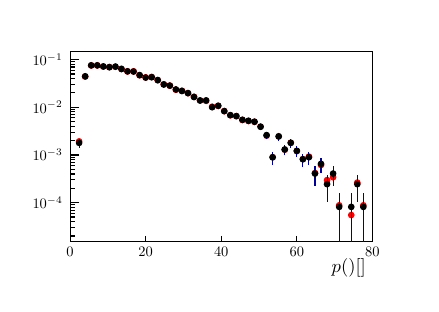
\begin{tikzpicture}
\pgfdeclareplotmark{cross} {
\pgfpathmoveto{\pgfpoint{-0.3\pgfplotmarksize}{\pgfplotmarksize}}
\pgfpathlineto{\pgfpoint{+0.3\pgfplotmarksize}{\pgfplotmarksize}}
\pgfpathlineto{\pgfpoint{+0.3\pgfplotmarksize}{0.3\pgfplotmarksize}}
\pgfpathlineto{\pgfpoint{+1\pgfplotmarksize}{0.3\pgfplotmarksize}}
\pgfpathlineto{\pgfpoint{+1\pgfplotmarksize}{-0.3\pgfplotmarksize}}
\pgfpathlineto{\pgfpoint{+0.3\pgfplotmarksize}{-0.3\pgfplotmarksize}}
\pgfpathlineto{\pgfpoint{+0.3\pgfplotmarksize}{-1.\pgfplotmarksize}}
\pgfpathlineto{\pgfpoint{-0.3\pgfplotmarksize}{-1.\pgfplotmarksize}}
\pgfpathlineto{\pgfpoint{-0.3\pgfplotmarksize}{-0.3\pgfplotmarksize}}
\pgfpathlineto{\pgfpoint{-1.\pgfplotmarksize}{-0.3\pgfplotmarksize}}
\pgfpathlineto{\pgfpoint{-1.\pgfplotmarksize}{0.3\pgfplotmarksize}}
\pgfpathlineto{\pgfpoint{-0.3\pgfplotmarksize}{0.3\pgfplotmarksize}}
\pgfpathclose
\pgfusepathqstroke
}
\pgfdeclareplotmark{cross*} {
\pgfpathmoveto{\pgfpoint{-0.3\pgfplotmarksize}{\pgfplotmarksize}}
\pgfpathlineto{\pgfpoint{+0.3\pgfplotmarksize}{\pgfplotmarksize}}
\pgfpathlineto{\pgfpoint{+0.3\pgfplotmarksize}{0.3\pgfplotmarksize}}
\pgfpathlineto{\pgfpoint{+1\pgfplotmarksize}{0.3\pgfplotmarksize}}
\pgfpathlineto{\pgfpoint{+1\pgfplotmarksize}{-0.3\pgfplotmarksize}}
\pgfpathlineto{\pgfpoint{+0.3\pgfplotmarksize}{-0.3\pgfplotmarksize}}
\pgfpathlineto{\pgfpoint{+0.3\pgfplotmarksize}{-1.\pgfplotmarksize}}
\pgfpathlineto{\pgfpoint{-0.3\pgfplotmarksize}{-1.\pgfplotmarksize}}
\pgfpathlineto{\pgfpoint{-0.3\pgfplotmarksize}{-0.3\pgfplotmarksize}}
\pgfpathlineto{\pgfpoint{-1.\pgfplotmarksize}{-0.3\pgfplotmarksize}}
\pgfpathlineto{\pgfpoint{-1.\pgfplotmarksize}{0.3\pgfplotmarksize}}
\pgfpathlineto{\pgfpoint{-0.3\pgfplotmarksize}{0.3\pgfplotmarksize}}
\pgfpathclose
\pgfusepathqfillstroke
}
\pgfdeclareplotmark{newstar} {
\pgfpathmoveto{\pgfqpoint{0pt}{\pgfplotmarksize}}
\pgfpathlineto{\pgfqpointpolar{44}{0.5\pgfplotmarksize}}
\pgfpathlineto{\pgfqpointpolar{18}{\pgfplotmarksize}}
\pgfpathlineto{\pgfqpointpolar{-20}{0.5\pgfplotmarksize}}
\pgfpathlineto{\pgfqpointpolar{-54}{\pgfplotmarksize}}
\pgfpathlineto{\pgfqpointpolar{-90}{0.5\pgfplotmarksize}}
\pgfpathlineto{\pgfqpointpolar{234}{\pgfplotmarksize}}
\pgfpathlineto{\pgfqpointpolar{198}{0.5\pgfplotmarksize}}
\pgfpathlineto{\pgfqpointpolar{162}{\pgfplotmarksize}}
\pgfpathlineto{\pgfqpointpolar{134}{0.5\pgfplotmarksize}}
\pgfpathclose
\pgfusepathqstroke
}
\pgfdeclareplotmark{newstar*} {
\pgfpathmoveto{\pgfqpoint{0pt}{\pgfplotmarksize}}
\pgfpathlineto{\pgfqpointpolar{44}{0.5\pgfplotmarksize}}
\pgfpathlineto{\pgfqpointpolar{18}{\pgfplotmarksize}}
\pgfpathlineto{\pgfqpointpolar{-20}{0.5\pgfplotmarksize}}
\pgfpathlineto{\pgfqpointpolar{-54}{\pgfplotmarksize}}
\pgfpathlineto{\pgfqpointpolar{-90}{0.5\pgfplotmarksize}}
\pgfpathlineto{\pgfqpointpolar{234}{\pgfplotmarksize}}
\pgfpathlineto{\pgfqpointpolar{198}{0.5\pgfplotmarksize}}
\pgfpathlineto{\pgfqpointpolar{162}{\pgfplotmarksize}}
\pgfpathlineto{\pgfqpointpolar{134}{0.5\pgfplotmarksize}}
\pgfpathclose
\pgfusepathqfillstroke
}
\definecolor{c}{rgb}{1,1,1};
\draw [color=c, fill=c] (0.1,0.0627517) rectangle (4.9,3.07483);
\draw [color=c, fill=c] (0.58,0.36396) rectangle (4.42,2.77362);
\definecolor{c}{rgb}{0,0,0};
\draw [c] (0.58,0.36396) -- (0.58,2.77362) -- (4.42,2.77362) -- (4.42,0.36396) -- (0.58,0.36396);
\definecolor{c}{rgb}{1,0,0};
\draw [c] (0.6952,1.61688) -- (0.6952,1.63756);
\draw [c] (0.6952,1.63756) -- (0.6952,1.65673);
\draw [c] (0.6568,1.63756) -- (0.6952,1.63756);
\draw [c] (0.6952,1.63756) -- (0.7336,1.63756);
\foreach \P in {(0.6952,1.63756)}{\draw[mark options={color=c,fill=c},mark size=2.402402pt,mark=*,mark size=1pt] plot coordinates {\P};}
\draw [c] (0.772,2.45646) -- (0.772,2.46065);
\draw [c] (0.772,2.46065) -- (0.772,2.46478);
\draw [c] (0.7336,2.46065) -- (0.772,2.46065);
\draw [c] (0.772,2.46065) -- (0.8104,2.46065);
\foreach \P in {(0.772,2.46065)}{\draw[mark options={color=c,fill=c},mark size=2.402402pt,mark=*,mark size=1pt] plot coordinates {\P};}
\draw [c] (0.8488,2.59887) -- (0.8488,2.60207);
\draw [c] (0.8488,2.60207) -- (0.8488,2.60523);
\draw [c] (0.8104,2.60207) -- (0.8488,2.60207);
\draw [c] (0.8488,2.60207) -- (0.8872,2.60207);
\foreach \P in {(0.8488,2.60207)}{\draw[mark options={color=c,fill=c},mark size=2.402402pt,mark=*,mark size=1pt] plot coordinates {\P};}
\draw [c] (0.9256,2.59914) -- (0.9256,2.60234);
\draw [c] (0.9256,2.60234) -- (0.9256,2.6055);
\draw [c] (0.8872,2.60234) -- (0.9256,2.60234);
\draw [c] (0.9256,2.60234) -- (0.964,2.60234);
\foreach \P in {(0.9256,2.60234)}{\draw[mark options={color=c,fill=c},mark size=2.402402pt,mark=*,mark size=1pt] plot coordinates {\P};}
\draw [c] (1.0024,2.58506) -- (1.0024,2.58834);
\draw [c] (1.0024,2.58834) -- (1.0024,2.59159);
\draw [c] (0.964,2.58834) -- (1.0024,2.58834);
\draw [c] (1.0024,2.58834) -- (1.0408,2.58834);
\foreach \P in {(1.0024,2.58834)}{\draw[mark options={color=c,fill=c},mark size=2.402402pt,mark=*,mark size=1pt] plot coordinates {\P};}
\draw [c] (1.0792,2.57929) -- (1.0792,2.58261);
\draw [c] (1.0792,2.58261) -- (1.0792,2.58589);
\draw [c] (1.0408,2.58261) -- (1.0792,2.58261);
\draw [c] (1.0792,2.58261) -- (1.1176,2.58261);
\foreach \P in {(1.0792,2.58261)}{\draw[mark options={color=c,fill=c},mark size=2.402402pt,mark=*,mark size=1pt] plot coordinates {\P};}
\draw [c] (1.156,2.58231) -- (1.156,2.58562);
\draw [c] (1.156,2.58562) -- (1.156,2.58888);
\draw [c] (1.1176,2.58562) -- (1.156,2.58562);
\draw [c] (1.156,2.58562) -- (1.1944,2.58562);
\foreach \P in {(1.156,2.58562)}{\draw[mark options={color=c,fill=c},mark size=2.402402pt,mark=*,mark size=1pt] plot coordinates {\P};}
\draw [c] (1.2328,2.55619) -- (1.2328,2.55966);
\draw [c] (1.2328,2.55966) -- (1.2328,2.56309);
\draw [c] (1.1944,2.55966) -- (1.2328,2.55966);
\draw [c] (1.2328,2.55966) -- (1.2712,2.55966);
\foreach \P in {(1.2328,2.55966)}{\draw[mark options={color=c,fill=c},mark size=2.402402pt,mark=*,mark size=1pt] plot coordinates {\P};}
\draw [c] (1.3096,2.52233) -- (1.3096,2.52603);
\draw [c] (1.3096,2.52603) -- (1.3096,2.52968);
\draw [c] (1.2712,2.52603) -- (1.3096,2.52603);
\draw [c] (1.3096,2.52603) -- (1.348,2.52603);
\foreach \P in {(1.3096,2.52603)}{\draw[mark options={color=c,fill=c},mark size=2.402402pt,mark=*,mark size=1pt] plot coordinates {\P};}
\draw [c] (1.3864,2.52326) -- (1.3864,2.52695);
\draw [c] (1.3864,2.52695) -- (1.3864,2.5306);
\draw [c] (1.348,2.52695) -- (1.3864,2.52695);
\draw [c] (1.3864,2.52695) -- (1.4248,2.52695);
\foreach \P in {(1.3864,2.52695)}{\draw[mark options={color=c,fill=c},mark size=2.402402pt,mark=*,mark size=1pt] plot coordinates {\P};}
\draw [c] (1.4632,2.4726) -- (1.4632,2.47667);
\draw [c] (1.4632,2.47667) -- (1.4632,2.48067);
\draw [c] (1.4248,2.47667) -- (1.4632,2.47667);
\draw [c] (1.4632,2.47667) -- (1.5016,2.47667);
\foreach \P in {(1.4632,2.47667)}{\draw[mark options={color=c,fill=c},mark size=2.402402pt,mark=*,mark size=1pt] plot coordinates {\P};}
\draw [c] (1.54,2.44652) -- (1.54,2.4508);
\draw [c] (1.54,2.4508) -- (1.54,2.455);
\draw [c] (1.5016,2.4508) -- (1.54,2.4508);
\draw [c] (1.54,2.4508) -- (1.5784,2.4508);
\foreach \P in {(1.54,2.4508)}{\draw[mark options={color=c,fill=c},mark size=2.402402pt,mark=*,mark size=1pt] plot coordinates {\P};}
\draw [c] (1.6168,2.45171) -- (1.6168,2.45594);
\draw [c] (1.6168,2.45594) -- (1.6168,2.4601);
\draw [c] (1.5784,2.45594) -- (1.6168,2.45594);
\draw [c] (1.6168,2.45594) -- (1.6552,2.45594);
\foreach \P in {(1.6168,2.45594)}{\draw[mark options={color=c,fill=c},mark size=2.402402pt,mark=*,mark size=1pt] plot coordinates {\P};}
\draw [c] (1.6936,2.40843) -- (1.6936,2.41303);
\draw [c] (1.6936,2.41303) -- (1.6936,2.41754);
\draw [c] (1.6552,2.41303) -- (1.6936,2.41303);
\draw [c] (1.6936,2.41303) -- (1.732,2.41303);
\foreach \P in {(1.6936,2.41303)}{\draw[mark options={color=c,fill=c},mark size=2.402402pt,mark=*,mark size=1pt] plot coordinates {\P};}
\draw [c] (1.7704,2.35821) -- (1.7704,2.36326);
\draw [c] (1.7704,2.36326) -- (1.7704,2.36822);
\draw [c] (1.732,2.36326) -- (1.7704,2.36326);
\draw [c] (1.7704,2.36326) -- (1.8088,2.36326);
\foreach \P in {(1.7704,2.36326)}{\draw[mark options={color=c,fill=c},mark size=2.402402pt,mark=*,mark size=1pt] plot coordinates {\P};}
\draw [c] (1.8472,2.33978) -- (1.8472,2.34502);
\draw [c] (1.8472,2.34502) -- (1.8472,2.35015);
\draw [c] (1.8088,2.34502) -- (1.8472,2.34502);
\draw [c] (1.8472,2.34502) -- (1.8856,2.34502);
\foreach \P in {(1.8472,2.34502)}{\draw[mark options={color=c,fill=c},mark size=2.402402pt,mark=*,mark size=1pt] plot coordinates {\P};}
\draw [c] (1.924,2.28774) -- (1.924,2.29352);
\draw [c] (1.924,2.29352) -- (1.924,2.29917);
\draw [c] (1.8856,2.29352) -- (1.924,2.29352);
\draw [c] (1.924,2.29352) -- (1.9624,2.29352);
\foreach \P in {(1.924,2.29352)}{\draw[mark options={color=c,fill=c},mark size=2.402402pt,mark=*,mark size=1pt] plot coordinates {\P};}
\draw [c] (2.0008,2.275) -- (2.0008,2.28092);
\draw [c] (2.0008,2.28092) -- (2.0008,2.28671);
\draw [c] (1.9624,2.28092) -- (2.0008,2.28092);
\draw [c] (2.0008,2.28092) -- (2.0392,2.28092);
\foreach \P in {(2.0008,2.28092)}{\draw[mark options={color=c,fill=c},mark size=2.402402pt,mark=*,mark size=1pt] plot coordinates {\P};}
\draw [c] (2.0776,2.24341) -- (2.0776,2.24969);
\draw [c] (2.0776,2.24969) -- (2.0776,2.25583);
\draw [c] (2.0392,2.24969) -- (2.0776,2.24969);
\draw [c] (2.0776,2.24969) -- (2.116,2.24969);
\foreach \P in {(2.0776,2.24969)}{\draw[mark options={color=c,fill=c},mark size=2.402402pt,mark=*,mark size=1pt] plot coordinates {\P};}
\draw [c] (2.1544,2.19747) -- (2.1544,2.20433);
\draw [c] (2.1544,2.20433) -- (2.1544,2.21101);
\draw [c] (2.116,2.20433) -- (2.1544,2.20433);
\draw [c] (2.1544,2.20433) -- (2.1928,2.20433);
\foreach \P in {(2.1544,2.20433)}{\draw[mark options={color=c,fill=c},mark size=2.402402pt,mark=*,mark size=1pt] plot coordinates {\P};}
\draw [c] (2.2312,2.15) -- (2.2312,2.15751);
\draw [c] (2.2312,2.15751) -- (2.2312,2.16481);
\draw [c] (2.1928,2.15751) -- (2.2312,2.15751);
\draw [c] (2.2312,2.15751) -- (2.2696,2.15751);
\foreach \P in {(2.2312,2.15751)}{\draw[mark options={color=c,fill=c},mark size=2.402402pt,mark=*,mark size=1pt] plot coordinates {\P};}
\draw [c] (2.308,2.14467) -- (2.308,2.15225);
\draw [c] (2.308,2.15225) -- (2.308,2.15963);
\draw [c] (2.2696,2.15225) -- (2.308,2.15225);
\draw [c] (2.308,2.15225) -- (2.3464,2.15225);
\foreach \P in {(2.308,2.15225)}{\draw[mark options={color=c,fill=c},mark size=2.402402pt,mark=*,mark size=1pt] plot coordinates {\P};}
\draw [c] (2.3848,2.06909) -- (2.3848,2.07784);
\draw [c] (2.3848,2.07784) -- (2.3848,2.08632);
\draw [c] (2.3464,2.07784) -- (2.3848,2.07784);
\draw [c] (2.3848,2.07784) -- (2.4232,2.07784);
\foreach \P in {(2.3848,2.07784)}{\draw[mark options={color=c,fill=c},mark size=2.402402pt,mark=*,mark size=1pt] plot coordinates {\P};}
\draw [c] (2.4616,2.07949) -- (2.4616,2.08807);
\draw [c] (2.4616,2.08807) -- (2.4616,2.09639);
\draw [c] (2.4232,2.08807) -- (2.4616,2.08807);
\draw [c] (2.4616,2.08807) -- (2.5,2.08807);
\foreach \P in {(2.4616,2.08807)}{\draw[mark options={color=c,fill=c},mark size=2.402402pt,mark=*,mark size=1pt] plot coordinates {\P};}
\draw [c] (2.5384,2.01169) -- (2.5384,2.02146);
\draw [c] (2.5384,2.02146) -- (2.5384,2.03087);
\draw [c] (2.5,2.02146) -- (2.5384,2.02146);
\draw [c] (2.5384,2.02146) -- (2.5768,2.02146);
\foreach \P in {(2.5384,2.02146)}{\draw[mark options={color=c,fill=c},mark size=2.402402pt,mark=*,mark size=1pt] plot coordinates {\P};}
\draw [c] (2.6152,1.95737) -- (2.6152,1.9682);
\draw [c] (2.6152,1.9682) -- (2.6152,1.9786);
\draw [c] (2.5768,1.9682) -- (2.6152,1.9682);
\draw [c] (2.6152,1.9682) -- (2.6536,1.9682);
\foreach \P in {(2.6152,1.9682)}{\draw[mark options={color=c,fill=c},mark size=2.402402pt,mark=*,mark size=1pt] plot coordinates {\P};}
\draw [c] (2.692,1.94759) -- (2.692,1.95862);
\draw [c] (2.692,1.95862) -- (2.692,1.9692);
\draw [c] (2.6536,1.95862) -- (2.692,1.95862);
\draw [c] (2.692,1.95862) -- (2.7304,1.95862);
\foreach \P in {(2.692,1.95862)}{\draw[mark options={color=c,fill=c},mark size=2.402402pt,mark=*,mark size=1pt] plot coordinates {\P};}
\draw [c] (2.7688,1.89736) -- (2.7688,1.9095);
\draw [c] (2.7688,1.9095) -- (2.7688,1.9211);
\draw [c] (2.7304,1.9095) -- (2.7688,1.9095);
\draw [c] (2.7688,1.9095) -- (2.8072,1.9095);
\foreach \P in {(2.7688,1.9095)}{\draw[mark options={color=c,fill=c},mark size=2.402402pt,mark=*,mark size=1pt] plot coordinates {\P};}
\draw [c] (2.8456,1.88389) -- (2.8456,1.89634);
\draw [c] (2.8456,1.89634) -- (2.8456,1.90823);
\draw [c] (2.8072,1.89634) -- (2.8456,1.89634);
\draw [c] (2.8456,1.89634) -- (2.884,1.89634);
\foreach \P in {(2.8456,1.89634)}{\draw[mark options={color=c,fill=c},mark size=2.402402pt,mark=*,mark size=1pt] plot coordinates {\P};}
\draw [c] (2.9224,1.87392) -- (2.9224,1.88661);
\draw [c] (2.9224,1.88661) -- (2.9224,1.89871);
\draw [c] (2.884,1.88661) -- (2.9224,1.88661);
\draw [c] (2.9224,1.88661) -- (2.9608,1.88661);
\foreach \P in {(2.9224,1.88661)}{\draw[mark options={color=c,fill=c},mark size=2.402402pt,mark=*,mark size=1pt] plot coordinates {\P};}
\draw [c] (2.9992,1.81006) -- (2.9992,1.82438);
\draw [c] (2.9992,1.82438) -- (2.9992,1.83797);
\draw [c] (2.9608,1.82438) -- (2.9992,1.82438);
\draw [c] (2.9992,1.82438) -- (3.0376,1.82438);
\foreach \P in {(2.9992,1.82438)}{\draw[mark options={color=c,fill=c},mark size=2.402402pt,mark=*,mark size=1pt] plot coordinates {\P};}
\draw [c] (3.076,1.69151) -- (3.076,1.70946);
\draw [c] (3.076,1.70946) -- (3.076,1.72626);
\draw [c] (3.0376,1.70946) -- (3.076,1.70946);
\draw [c] (3.076,1.70946) -- (3.1144,1.70946);
\foreach \P in {(3.076,1.70946)}{\draw[mark options={color=c,fill=c},mark size=2.402402pt,mark=*,mark size=1pt] plot coordinates {\P};}
\draw [c] (3.1528,1.40392) -- (3.1528,1.43491);
\draw [c] (3.1528,1.43491) -- (3.1528,1.46263);
\draw [c] (3.1144,1.43491) -- (3.1528,1.43491);
\draw [c] (3.1528,1.43491) -- (3.1912,1.43491);
\foreach \P in {(3.1528,1.43491)}{\draw[mark options={color=c,fill=c},mark size=2.402402pt,mark=*,mark size=1pt] plot coordinates {\P};}
\draw [c] (3.2296,1.68431) -- (3.2296,1.7025);
\draw [c] (3.2296,1.7025) -- (3.2296,1.71952);
\draw [c] (3.1912,1.7025) -- (3.2296,1.7025);
\draw [c] (3.2296,1.7025) -- (3.268,1.7025);
\foreach \P in {(3.2296,1.7025)}{\draw[mark options={color=c,fill=c},mark size=2.402402pt,mark=*,mark size=1pt] plot coordinates {\P};}
\draw [c] (3.3064,1.50613) -- (3.3064,1.53165);
\draw [c] (3.3064,1.53165) -- (3.3064,1.55491);
\draw [c] (3.268,1.53165) -- (3.3064,1.53165);
\draw [c] (3.3064,1.53165) -- (3.3448,1.53165);
\foreach \P in {(3.3064,1.53165)}{\draw[mark options={color=c,fill=c},mark size=2.402402pt,mark=*,mark size=1pt] plot coordinates {\P};}
\draw [c] (3.3832,1.59909) -- (3.3832,1.62048);
\draw [c] (3.3832,1.62048) -- (3.3832,1.64026);
\draw [c] (3.3448,1.62048) -- (3.3832,1.62048);
\draw [c] (3.3832,1.62048) -- (3.4216,1.62048);
\foreach \P in {(3.3832,1.62048)}{\draw[mark options={color=c,fill=c},mark size=2.402402pt,mark=*,mark size=1pt] plot coordinates {\P};}
\draw [c] (3.46,1.48653) -- (3.46,1.51301);
\draw [c] (3.46,1.51301) -- (3.46,1.53708);
\draw [c] (3.4216,1.51301) -- (3.46,1.51301);
\draw [c] (3.46,1.51301) -- (3.4984,1.51301);
\foreach \P in {(3.46,1.51301)}{\draw[mark options={color=c,fill=c},mark size=2.402402pt,mark=*,mark size=1pt] plot coordinates {\P};}
\draw [c] (3.5368,1.37862) -- (3.5368,1.41113);
\draw [c] (3.5368,1.41113) -- (3.5368,1.44006);
\draw [c] (3.4984,1.41113) -- (3.5368,1.41113);
\draw [c] (3.5368,1.41113) -- (3.5752,1.41113);
\foreach \P in {(3.5368,1.41113)}{\draw[mark options={color=c,fill=c},mark size=2.402402pt,mark=*,mark size=1pt] plot coordinates {\P};}
\draw [c] (3.6136,1.41408) -- (3.6136,1.44448);
\draw [c] (3.6136,1.44448) -- (3.6136,1.47172);
\draw [c] (3.5752,1.44448) -- (3.6136,1.44448);
\draw [c] (3.6136,1.44448) -- (3.652,1.44448);
\foreach \P in {(3.6136,1.44448)}{\draw[mark options={color=c,fill=c},mark size=2.402402pt,mark=*,mark size=1pt] plot coordinates {\P};}
\draw [c] (3.6904,1.18924) -- (3.6904,1.2358);
\draw [c] (3.6904,1.2358) -- (3.6904,1.27535);
\draw [c] (3.652,1.2358) -- (3.6904,1.2358);
\draw [c] (3.6904,1.2358) -- (3.7288,1.2358);
\foreach \P in {(3.6904,1.2358)}{\draw[mark options={color=c,fill=c},mark size=2.402402pt,mark=*,mark size=1pt] plot coordinates {\P};}
\draw [c] (3.7672,1.30007) -- (3.7672,1.33781);
\draw [c] (3.7672,1.33781) -- (3.7672,1.37081);
\draw [c] (3.7288,1.33781) -- (3.7672,1.33781);
\draw [c] (3.7672,1.33781) -- (3.8056,1.33781);
\foreach \P in {(3.7672,1.33781)}{\draw[mark options={color=c,fill=c},mark size=2.402402pt,mark=*,mark size=1pt] plot coordinates {\P};}
\draw [c] (3.844,1.08966) -- (3.844,1.1459);
\draw [c] (3.844,1.1459) -- (3.844,1.1922);
\draw [c] (3.8056,1.1459) -- (3.844,1.1459);
\draw [c] (3.844,1.1459) -- (3.8824,1.1459);
\foreach \P in {(3.844,1.1459)}{\draw[mark options={color=c,fill=c},mark size=2.402402pt,mark=*,mark size=1pt] plot coordinates {\P};}
\draw [c] (3.9208,1.13016) -- (3.9208,1.18224);
\draw [c] (3.9208,1.18224) -- (3.9208,1.22569);
\draw [c] (3.8824,1.18224) -- (3.9208,1.18224);
\draw [c] (3.9208,1.18224) -- (3.9592,1.18224);
\foreach \P in {(3.9208,1.18224)}{\draw[mark options={color=c,fill=c},mark size=2.402402pt,mark=*,mark size=1pt] plot coordinates {\P};}
\draw [c] (3.9976,0.711127) -- (3.9976,0.825896);
\draw [c] (3.9976,0.825896) -- (3.9976,0.905537);
\draw [c] (3.9592,0.825896) -- (3.9976,0.825896);
\draw [c] (3.9976,0.825896) -- (4.036,0.825896);
\foreach \P in {(3.9976,0.825896)}{\draw[mark options={color=c,fill=c},mark size=2.402402pt,mark=*,mark size=1pt] plot coordinates {\P};}
\draw [c] (4.1512,0.546307) -- (4.1512,0.702251);
\draw [c] (4.1512,0.702251) -- (4.1512,0.799493);
\draw [c] (4.1128,0.702251) -- (4.1512,0.702251);
\draw [c] (4.1512,0.702251) -- (4.1896,0.702251);
\foreach \P in {(4.1512,0.702251)}{\draw[mark options={color=c,fill=c},mark size=2.402402pt,mark=*,mark size=1pt] plot coordinates {\P};}
\draw [c] (4.228,1.05485) -- (4.228,1.11491);
\draw [c] (4.228,1.11491) -- (4.228,1.16378);
\draw [c] (4.1896,1.11491) -- (4.228,1.11491);
\draw [c] (4.228,1.11491) -- (4.2664,1.11491);
\foreach \P in {(4.228,1.11491)}{\draw[mark options={color=c,fill=c},mark size=2.402402pt,mark=*,mark size=1pt] plot coordinates {\P};}
\draw [c] (4.3048,0.711127) -- (4.3048,0.825896);
\draw [c] (4.3048,0.825896) -- (4.3048,0.905537);
\draw [c] (4.2664,0.825896) -- (4.3048,0.825896);
\draw [c] (4.3048,0.825896) -- (4.3432,0.825896);
\foreach \P in {(4.3048,0.825896)}{\draw[mark options={color=c,fill=c},mark size=2.402402pt,mark=*,mark size=1pt] plot coordinates {\P};}
\definecolor{c}{rgb}{0,0,0};
\draw [c] (0.58,0.36396) -- (4.42,0.36396);
\draw [anchor= east] (4.42,0.0266067) node[scale=0.672711, rotate=0]{$p(\kaon) [\mevc]$};
\draw [c] (0.58,0.43625) -- (0.58,0.36396);
\draw [c] (1.54,0.43625) -- (1.54,0.36396);
\draw [c] (2.5,0.43625) -- (2.5,0.36396);
\draw [c] (3.46,0.43625) -- (3.46,0.36396);
\draw [c] (4.42,0.43625) -- (4.42,0.36396);
\draw [anchor=base] (0.58,0.171187) node[scale=0.52322, rotate=0]{0};
\draw [anchor=base] (1.54,0.171187) node[scale=0.52322, rotate=0]{20};
\draw [anchor=base] (2.5,0.171187) node[scale=0.52322, rotate=0]{40};
\draw [anchor=base] (3.46,0.171187) node[scale=0.52322, rotate=0]{60};
\draw [anchor=base] (4.42,0.171187) node[scale=0.52322, rotate=0]{80};
\draw [c] (0.58,0.36396) -- (0.58,2.77362);
\draw [c] (0.6376,0.435798) -- (0.58,0.435798);
\draw [c] (0.6376,0.542465) -- (0.58,0.542465);
\draw [c] (0.6376,0.618146) -- (0.58,0.618146);
\draw [c] (0.6376,0.676848) -- (0.58,0.676848);
\draw [c] (0.6376,0.724812) -- (0.58,0.724812);
\draw [c] (0.6376,0.765365) -- (0.58,0.765365);
\draw [c] (0.6376,0.800493) -- (0.58,0.800493);
\draw [c] (0.6376,0.831478) -- (0.58,0.831478);
\draw [c] (0.6952,0.859196) -- (0.58,0.859196);
\draw [anchor= east] (0.54928,0.859196) node[scale=0.52322, rotate=0]{$10^{-4}$};
\draw [c] (0.6376,1.04154) -- (0.58,1.04154);
\draw [c] (0.6376,1.14821) -- (0.58,1.14821);
\draw [c] (0.6376,1.22389) -- (0.58,1.22389);
\draw [c] (0.6376,1.28259) -- (0.58,1.28259);
\draw [c] (0.6376,1.33056) -- (0.58,1.33056);
\draw [c] (0.6376,1.37111) -- (0.58,1.37111);
\draw [c] (0.6376,1.40624) -- (0.58,1.40624);
\draw [c] (0.6376,1.43722) -- (0.58,1.43722);
\draw [c] (0.6952,1.46494) -- (0.58,1.46494);
\draw [anchor= east] (0.54928,1.46494) node[scale=0.52322, rotate=0]{$10^{-3}$};
\draw [c] (0.6376,1.64729) -- (0.58,1.64729);
\draw [c] (0.6376,1.75395) -- (0.58,1.75395);
\draw [c] (0.6376,1.82963) -- (0.58,1.82963);
\draw [c] (0.6376,1.88834) -- (0.58,1.88834);
\draw [c] (0.6376,1.9363) -- (0.58,1.9363);
\draw [c] (0.6376,1.97685) -- (0.58,1.97685);
\draw [c] (0.6376,2.01198) -- (0.58,2.01198);
\draw [c] (0.6376,2.04297) -- (0.58,2.04297);
\draw [c] (0.6952,2.07068) -- (0.58,2.07068);
\draw [anchor= east] (0.54928,2.07068) node[scale=0.52322, rotate=0]{$10^{-2}$};
\draw [c] (0.6376,2.25303) -- (0.58,2.25303);
\draw [c] (0.6376,2.3597) -- (0.58,2.3597);
\draw [c] (0.6376,2.43538) -- (0.58,2.43538);
\draw [c] (0.6376,2.49408) -- (0.58,2.49408);
\draw [c] (0.6376,2.54204) -- (0.58,2.54204);
\draw [c] (0.6376,2.5826) -- (0.58,2.5826);
\draw [c] (0.6376,2.61773) -- (0.58,2.61773);
\draw [c] (0.6376,2.64871) -- (0.58,2.64871);
\draw [c] (0.6952,2.67643) -- (0.58,2.67643);
\draw [anchor= east] (0.54928,2.67643) node[scale=0.52322, rotate=0]{$10^{-1}$};
\definecolor{c}{rgb}{0,0,0.6};
\draw [c] (0.6952,1.55576) -- (0.6952,1.61884);
\draw [c] (0.6952,1.61884) -- (0.6952,1.66969);
\draw [c] (0.6568,1.61884) -- (0.6952,1.61884);
\draw [c] (0.6952,1.61884) -- (0.7336,1.61884);
\definecolor{c}{rgb}{0,0,0};
\foreach \P in {(0.6952,1.61884)}{\draw[mark options={color=c,fill=c},mark size=2.402402pt,mark=*,mark size=1pt] plot coordinates {\P};}
\definecolor{c}{rgb}{0,0,0.6};
\draw [c] (0.772,2.4527) -- (0.772,2.4642);
\draw [c] (0.772,2.4642) -- (0.772,2.47521);
\draw [c] (0.7336,2.4642) -- (0.772,2.4642);
\draw [c] (0.772,2.4642) -- (0.8104,2.4642);
\definecolor{c}{rgb}{0,0,0};
\foreach \P in {(0.772,2.4642)}{\draw[mark options={color=c,fill=c},mark size=2.402402pt,mark=*,mark size=1pt] plot coordinates {\P};}
\definecolor{c}{rgb}{0,0,0.6};
\draw [c] (0.8488,2.59447) -- (0.8488,2.60325);
\draw [c] (0.8488,2.60325) -- (0.8488,2.61175);
\draw [c] (0.8104,2.60325) -- (0.8488,2.60325);
\draw [c] (0.8488,2.60325) -- (0.8872,2.60325);
\definecolor{c}{rgb}{0,0,0};
\foreach \P in {(0.8488,2.60325)}{\draw[mark options={color=c,fill=c},mark size=2.402402pt,mark=*,mark size=1pt] plot coordinates {\P};}
\definecolor{c}{rgb}{0,0,0.6};
\draw [c] (0.9256,2.59447) -- (0.9256,2.60325);
\draw [c] (0.9256,2.60325) -- (0.9256,2.61175);
\draw [c] (0.8872,2.60325) -- (0.9256,2.60325);
\draw [c] (0.9256,2.60325) -- (0.964,2.60325);
\definecolor{c}{rgb}{0,0,0};
\foreach \P in {(0.9256,2.60325)}{\draw[mark options={color=c,fill=c},mark size=2.402402pt,mark=*,mark size=1pt] plot coordinates {\P};}
\definecolor{c}{rgb}{0,0,0.6};
\draw [c] (1.0024,2.58057) -- (1.0024,2.58958);
\draw [c] (1.0024,2.58958) -- (1.0024,2.5983);
\draw [c] (0.964,2.58958) -- (1.0024,2.58958);
\draw [c] (1.0024,2.58958) -- (1.0408,2.58958);
\definecolor{c}{rgb}{0,0,0};
\foreach \P in {(1.0024,2.58958)}{\draw[mark options={color=c,fill=c},mark size=2.402402pt,mark=*,mark size=1pt] plot coordinates {\P};}
\definecolor{c}{rgb}{0,0,0.6};
\draw [c] (1.0792,2.57003) -- (1.0792,2.57923);
\draw [c] (1.0792,2.57923) -- (1.0792,2.58811);
\draw [c] (1.0408,2.57923) -- (1.0792,2.57923);
\draw [c] (1.0792,2.57923) -- (1.1176,2.57923);
\definecolor{c}{rgb}{0,0,0};
\foreach \P in {(1.0792,2.57923)}{\draw[mark options={color=c,fill=c},mark size=2.402402pt,mark=*,mark size=1pt] plot coordinates {\P};}
\definecolor{c}{rgb}{0,0,0.6};
\draw [c] (1.156,2.57843) -- (1.156,2.58748);
\draw [c] (1.156,2.58748) -- (1.156,2.59623);
\draw [c] (1.1176,2.58748) -- (1.156,2.58748);
\draw [c] (1.156,2.58748) -- (1.1944,2.58748);
\definecolor{c}{rgb}{0,0,0};
\foreach \P in {(1.156,2.58748)}{\draw[mark options={color=c,fill=c},mark size=2.402402pt,mark=*,mark size=1pt] plot coordinates {\P};}
\definecolor{c}{rgb}{0,0,0.6};
\draw [c] (1.2328,2.54658) -- (1.2328,2.5562);
\draw [c] (1.2328,2.5562) -- (1.2328,2.56547);
\draw [c] (1.1944,2.5562) -- (1.2328,2.5562);
\draw [c] (1.2328,2.5562) -- (1.2712,2.5562);
\definecolor{c}{rgb}{0,0,0};
\foreach \P in {(1.2328,2.5562)}{\draw[mark options={color=c,fill=c},mark size=2.402402pt,mark=*,mark size=1pt] plot coordinates {\P};}
\definecolor{c}{rgb}{0,0,0.6};
\draw [c] (1.3096,2.51702) -- (1.3096,2.52719);
\draw [c] (1.3096,2.52719) -- (1.3096,2.53699);
\draw [c] (1.2712,2.52719) -- (1.3096,2.52719);
\draw [c] (1.3096,2.52719) -- (1.348,2.52719);
\definecolor{c}{rgb}{0,0,0};
\foreach \P in {(1.3096,2.52719)}{\draw[mark options={color=c,fill=c},mark size=2.402402pt,mark=*,mark size=1pt] plot coordinates {\P};}
\definecolor{c}{rgb}{0,0,0.6};
\draw [c] (1.3864,2.51431) -- (1.3864,2.52453);
\draw [c] (1.3864,2.52453) -- (1.3864,2.53437);
\draw [c] (1.348,2.52453) -- (1.3864,2.52453);
\draw [c] (1.3864,2.52453) -- (1.4248,2.52453);
\definecolor{c}{rgb}{0,0,0};
\foreach \P in {(1.3864,2.52453)}{\draw[mark options={color=c,fill=c},mark size=2.402402pt,mark=*,mark size=1pt] plot coordinates {\P};}
\definecolor{c}{rgb}{0,0,0.6};
\draw [c] (1.4632,2.46845) -- (1.4632,2.47961);
\draw [c] (1.4632,2.47961) -- (1.4632,2.49031);
\draw [c] (1.4248,2.47961) -- (1.4632,2.47961);
\draw [c] (1.4632,2.47961) -- (1.5016,2.47961);
\definecolor{c}{rgb}{0,0,0};
\foreach \P in {(1.4632,2.47961)}{\draw[mark options={color=c,fill=c},mark size=2.402402pt,mark=*,mark size=1pt] plot coordinates {\P};}
\definecolor{c}{rgb}{0,0,0.6};
\draw [c] (1.54,2.43596) -- (1.54,2.44783);
\draw [c] (1.54,2.44783) -- (1.54,2.45918);
\draw [c] (1.5016,2.44783) -- (1.54,2.44783);
\draw [c] (1.54,2.44783) -- (1.5784,2.44783);
\definecolor{c}{rgb}{0,0,0};
\foreach \P in {(1.54,2.44783)}{\draw[mark options={color=c,fill=c},mark size=2.402402pt,mark=*,mark size=1pt] plot coordinates {\P};}
\definecolor{c}{rgb}{0,0,0.6};
\draw [c] (1.6168,2.44063) -- (1.6168,2.4524);
\draw [c] (1.6168,2.4524) -- (1.6168,2.46365);
\draw [c] (1.5784,2.4524) -- (1.6168,2.4524);
\draw [c] (1.6168,2.4524) -- (1.6552,2.4524);
\definecolor{c}{rgb}{0,0,0};
\foreach \P in {(1.6168,2.4524)}{\draw[mark options={color=c,fill=c},mark size=2.402402pt,mark=*,mark size=1pt] plot coordinates {\P};}
\definecolor{c}{rgb}{0,0,0.6};
\draw [c] (1.6936,2.4043) -- (1.6936,2.41691);
\draw [c] (1.6936,2.41691) -- (1.6936,2.42893);
\draw [c] (1.6552,2.41691) -- (1.6936,2.41691);
\draw [c] (1.6936,2.41691) -- (1.732,2.41691);
\definecolor{c}{rgb}{0,0,0};
\foreach \P in {(1.6936,2.41691)}{\draw[mark options={color=c,fill=c},mark size=2.402402pt,mark=*,mark size=1pt] plot coordinates {\P};}
\definecolor{c}{rgb}{0,0,0.6};
\draw [c] (1.7704,2.34584) -- (1.7704,2.35993);
\draw [c] (1.7704,2.35993) -- (1.7704,2.37329);
\draw [c] (1.732,2.35993) -- (1.7704,2.35993);
\draw [c] (1.7704,2.35993) -- (1.8088,2.35993);
\definecolor{c}{rgb}{0,0,0};
\foreach \P in {(1.7704,2.35993)}{\draw[mark options={color=c,fill=c},mark size=2.402402pt,mark=*,mark size=1pt] plot coordinates {\P};}
\definecolor{c}{rgb}{0,0,0.6};
\draw [c] (1.8472,2.33151) -- (1.8472,2.34598);
\draw [c] (1.8472,2.34598) -- (1.8472,2.3597);
\draw [c] (1.8088,2.34598) -- (1.8472,2.34598);
\draw [c] (1.8472,2.34598) -- (1.8856,2.34598);
\definecolor{c}{rgb}{0,0,0};
\foreach \P in {(1.8472,2.34598)}{\draw[mark options={color=c,fill=c},mark size=2.402402pt,mark=*,mark size=1pt] plot coordinates {\P};}
\definecolor{c}{rgb}{0,0,0.6};
\draw [c] (1.924,2.28134) -- (1.924,2.29726);
\draw [c] (1.924,2.29726) -- (1.924,2.31227);
\draw [c] (1.8856,2.29726) -- (1.924,2.29726);
\draw [c] (1.924,2.29726) -- (1.9624,2.29726);
\definecolor{c}{rgb}{0,0,0};
\foreach \P in {(1.924,2.29726)}{\draw[mark options={color=c,fill=c},mark size=2.402402pt,mark=*,mark size=1pt] plot coordinates {\P};}
\definecolor{c}{rgb}{0,0,0.6};
\draw [c] (2.0008,2.26094) -- (2.0008,2.27749);
\draw [c] (2.0008,2.27749) -- (2.0008,2.29306);
\draw [c] (1.9624,2.27749) -- (2.0008,2.27749);
\draw [c] (2.0008,2.27749) -- (2.0392,2.27749);
\definecolor{c}{rgb}{0,0,0};
\foreach \P in {(2.0008,2.27749)}{\draw[mark options={color=c,fill=c},mark size=2.402402pt,mark=*,mark size=1pt] plot coordinates {\P};}
\definecolor{c}{rgb}{0,0,0.6};
\draw [c] (2.0776,2.2333) -- (2.0776,2.25075);
\draw [c] (2.0776,2.25075) -- (2.0776,2.2671);
\draw [c] (2.0392,2.25075) -- (2.0776,2.25075);
\draw [c] (2.0776,2.25075) -- (2.116,2.25075);
\definecolor{c}{rgb}{0,0,0};
\foreach \P in {(2.0776,2.25075)}{\draw[mark options={color=c,fill=c},mark size=2.402402pt,mark=*,mark size=1pt] plot coordinates {\P};}
\definecolor{c}{rgb}{0,0,0.6};
\draw [c] (2.1544,2.18158) -- (2.1544,2.20083);
\draw [c] (2.1544,2.20083) -- (2.1544,2.21876);
\draw [c] (2.116,2.20083) -- (2.1544,2.20083);
\draw [c] (2.1544,2.20083) -- (2.1928,2.20083);
\definecolor{c}{rgb}{0,0,0};
\foreach \P in {(2.1544,2.20083)}{\draw[mark options={color=c,fill=c},mark size=2.402402pt,mark=*,mark size=1pt] plot coordinates {\P};}
\definecolor{c}{rgb}{0,0,0.6};
\draw [c] (2.2312,2.13577) -- (2.2312,2.15676);
\draw [c] (2.2312,2.15676) -- (2.2312,2.1762);
\draw [c] (2.1928,2.15676) -- (2.2312,2.15676);
\draw [c] (2.2312,2.15676) -- (2.2696,2.15676);
\definecolor{c}{rgb}{0,0,0};
\foreach \P in {(2.2312,2.15676)}{\draw[mark options={color=c,fill=c},mark size=2.402402pt,mark=*,mark size=1pt] plot coordinates {\P};}
\definecolor{c}{rgb}{0,0,0.6};
\draw [c] (2.308,2.13738) -- (2.308,2.1583);
\draw [c] (2.308,2.1583) -- (2.308,2.17769);
\draw [c] (2.2696,2.1583) -- (2.308,2.1583);
\draw [c] (2.308,2.1583) -- (2.3464,2.1583);
\definecolor{c}{rgb}{0,0,0};
\foreach \P in {(2.308,2.1583)}{\draw[mark options={color=c,fill=c},mark size=2.402402pt,mark=*,mark size=1pt] plot coordinates {\P};}
\definecolor{c}{rgb}{0,0,0.6};
\draw [c] (2.3848,2.04677) -- (2.3848,2.07163);
\draw [c] (2.3848,2.07163) -- (2.3848,2.09434);
\draw [c] (2.3464,2.07163) -- (2.3848,2.07163);
\draw [c] (2.3848,2.07163) -- (2.4232,2.07163);
\definecolor{c}{rgb}{0,0,0};
\foreach \P in {(2.3848,2.07163)}{\draw[mark options={color=c,fill=c},mark size=2.402402pt,mark=*,mark size=1pt] plot coordinates {\P};}
\definecolor{c}{rgb}{0,0,0.6};
\draw [c] (2.4616,2.06625) -- (2.4616,2.0902);
\draw [c] (2.4616,2.0902) -- (2.4616,2.11216);
\draw [c] (2.4232,2.0902) -- (2.4616,2.0902);
\draw [c] (2.4616,2.0902) -- (2.5,2.0902);
\definecolor{c}{rgb}{0,0,0};
\foreach \P in {(2.4616,2.0902)}{\draw[mark options={color=c,fill=c},mark size=2.402402pt,mark=*,mark size=1pt] plot coordinates {\P};}
\definecolor{c}{rgb}{0,0,0.6};
\draw [c] (2.5384,1.99495) -- (2.5384,2.02238);
\draw [c] (2.5384,2.02238) -- (2.5384,2.04721);
\draw [c] (2.5,2.02238) -- (2.5384,2.02238);
\draw [c] (2.5384,2.02238) -- (2.5768,2.02238);
\definecolor{c}{rgb}{0,0,0};
\foreach \P in {(2.5384,2.02238)}{\draw[mark options={color=c,fill=c},mark size=2.402402pt,mark=*,mark size=1pt] plot coordinates {\P};}
\definecolor{c}{rgb}{0,0,0.6};
\draw [c] (2.6152,1.94091) -- (2.6152,1.9713);
\draw [c] (2.6152,1.9713) -- (2.6152,1.99854);
\draw [c] (2.5768,1.9713) -- (2.6152,1.9713);
\draw [c] (2.6152,1.9713) -- (2.6536,1.9713);
\definecolor{c}{rgb}{0,0,0};
\foreach \P in {(2.6152,1.9713)}{\draw[mark options={color=c,fill=c},mark size=2.402402pt,mark=*,mark size=1pt] plot coordinates {\P};}
\definecolor{c}{rgb}{0,0,0.6};
\draw [c] (2.692,1.92727) -- (2.692,1.95846);
\draw [c] (2.692,1.95846) -- (2.692,1.98635);
\draw [c] (2.6536,1.95846) -- (2.692,1.95846);
\draw [c] (2.692,1.95846) -- (2.7304,1.95846);
\definecolor{c}{rgb}{0,0,0};
\foreach \P in {(2.692,1.95846)}{\draw[mark options={color=c,fill=c},mark size=2.402402pt,mark=*,mark size=1pt] plot coordinates {\P};}
\definecolor{c}{rgb}{0,0,0.6};
\draw [c] (2.7688,1.87753) -- (2.7688,1.91181);
\draw [c] (2.7688,1.91181) -- (2.7688,1.94214);
\draw [c] (2.7304,1.91181) -- (2.7688,1.91181);
\draw [c] (2.7688,1.91181) -- (2.8072,1.91181);
\definecolor{c}{rgb}{0,0,0};
\foreach \P in {(2.7688,1.91181)}{\draw[mark options={color=c,fill=c},mark size=2.402402pt,mark=*,mark size=1pt] plot coordinates {\P};}
\definecolor{c}{rgb}{0,0,0.6};
\draw [c] (2.8456,1.86463) -- (2.8456,1.89976);
\draw [c] (2.8456,1.89976) -- (2.8456,1.93075);
\draw [c] (2.8072,1.89976) -- (2.8456,1.89976);
\draw [c] (2.8456,1.89976) -- (2.884,1.89976);
\definecolor{c}{rgb}{0,0,0};
\foreach \P in {(2.8456,1.89976)}{\draw[mark options={color=c,fill=c},mark size=2.402402pt,mark=*,mark size=1pt] plot coordinates {\P};}
\definecolor{c}{rgb}{0,0,0.6};
\draw [c] (2.9224,1.85109) -- (2.9224,1.88713);
\draw [c] (2.9224,1.88713) -- (2.9224,1.91883);
\draw [c] (2.884,1.88713) -- (2.9224,1.88713);
\draw [c] (2.9224,1.88713) -- (2.9608,1.88713);
\definecolor{c}{rgb}{0,0,0};
\foreach \P in {(2.9224,1.88713)}{\draw[mark options={color=c,fill=c},mark size=2.402402pt,mark=*,mark size=1pt] plot coordinates {\P};}
\definecolor{c}{rgb}{0,0,0.6};
\draw [c] (2.9992,1.78307) -- (2.9992,1.82408);
\draw [c] (2.9992,1.82408) -- (2.9992,1.85955);
\draw [c] (2.9608,1.82408) -- (2.9992,1.82408);
\draw [c] (2.9992,1.82408) -- (3.0376,1.82408);
\definecolor{c}{rgb}{0,0,0};
\foreach \P in {(2.9992,1.82408)}{\draw[mark options={color=c,fill=c},mark size=2.402402pt,mark=*,mark size=1pt] plot coordinates {\P};}
\definecolor{c}{rgb}{0,0,0.6};
\draw [c] (3.076,1.66624) -- (3.076,1.71741);
\draw [c] (3.076,1.71741) -- (3.076,1.76024);
\draw [c] (3.0376,1.71741) -- (3.076,1.71741);
\draw [c] (3.076,1.71741) -- (3.1144,1.71741);
\definecolor{c}{rgb}{0,0,0};
\foreach \P in {(3.076,1.71741)}{\draw[mark options={color=c,fill=c},mark size=2.402402pt,mark=*,mark size=1pt] plot coordinates {\P};}
\definecolor{c}{rgb}{0,0,0.6};
\draw [c] (3.1528,1.3421) -- (3.1528,1.4365);
\draw [c] (3.1528,1.4365) -- (3.1528,1.50582);
\draw [c] (3.1144,1.4365) -- (3.1528,1.4365);
\draw [c] (3.1528,1.4365) -- (3.1912,1.4365);
\definecolor{c}{rgb}{0,0,0};
\foreach \P in {(3.1528,1.4365)}{\draw[mark options={color=c,fill=c},mark size=2.402402pt,mark=*,mark size=1pt] plot coordinates {\P};}
\definecolor{c}{rgb}{0,0,0.6};
\draw [c] (3.2296,1.6474) -- (3.2296,1.70044);
\draw [c] (3.2296,1.70044) -- (3.2296,1.74455);
\draw [c] (3.1912,1.70044) -- (3.2296,1.70044);
\draw [c] (3.2296,1.70044) -- (3.268,1.70044);
\definecolor{c}{rgb}{0,0,0};
\foreach \P in {(3.2296,1.70044)}{\draw[mark options={color=c,fill=c},mark size=2.402402pt,mark=*,mark size=1pt] plot coordinates {\P};}
\definecolor{c}{rgb}{0,0,0.6};
\draw [c] (3.3064,1.45939) -- (3.3064,1.53507);
\draw [c] (3.3064,1.53507) -- (3.3064,1.59377);
\draw [c] (3.268,1.53507) -- (3.3064,1.53507);
\draw [c] (3.3064,1.53507) -- (3.3448,1.53507);
\definecolor{c}{rgb}{0,0,0};
\foreach \P in {(3.3064,1.53507)}{\draw[mark options={color=c,fill=c},mark size=2.402402pt,mark=*,mark size=1pt] plot coordinates {\P};}
\definecolor{c}{rgb}{0,0,0.6};
\draw [c] (3.3832,1.55576) -- (3.3832,1.61884);
\draw [c] (3.3832,1.61884) -- (3.3832,1.66969);
\draw [c] (3.3448,1.61884) -- (3.3832,1.61884);
\draw [c] (3.3832,1.61884) -- (3.4216,1.61884);
\definecolor{c}{rgb}{0,0,0};
\foreach \P in {(3.3832,1.61884)}{\draw[mark options={color=c,fill=c},mark size=2.402402pt,mark=*,mark size=1pt] plot coordinates {\P};}
\definecolor{c}{rgb}{0,0,0.6};
\draw [c] (3.46,1.43952) -- (3.46,1.51809);
\draw [c] (3.46,1.51809) -- (3.46,1.57851);
\draw [c] (3.4216,1.51809) -- (3.46,1.51809);
\draw [c] (3.46,1.51809) -- (3.4984,1.51809);
\definecolor{c}{rgb}{0,0,0};
\foreach \P in {(3.46,1.51809)}{\draw[mark options={color=c,fill=c},mark size=2.402402pt,mark=*,mark size=1pt] plot coordinates {\P};}
\definecolor{c}{rgb}{0,0,0.6};
\draw [c] (3.5368,1.31142) -- (3.5368,1.41142);
\draw [c] (3.5368,1.41142) -- (3.5368,1.48371);
\draw [c] (3.4984,1.41142) -- (3.5368,1.41142);
\draw [c] (3.5368,1.41142) -- (3.5752,1.41142);
\definecolor{c}{rgb}{0,0,0};
\foreach \P in {(3.5368,1.41142)}{\draw[mark options={color=c,fill=c},mark size=2.402402pt,mark=*,mark size=1pt] plot coordinates {\P};}
\definecolor{c}{rgb}{0,0,0.6};
\draw [c] (3.6136,1.3421) -- (3.6136,1.4365);
\draw [c] (3.6136,1.4365) -- (3.6136,1.50582);
\draw [c] (3.5752,1.4365) -- (3.6136,1.4365);
\draw [c] (3.6136,1.4365) -- (3.652,1.4365);
\definecolor{c}{rgb}{0,0,0};
\foreach \P in {(3.6136,1.4365)}{\draw[mark options={color=c,fill=c},mark size=2.402402pt,mark=*,mark size=1pt] plot coordinates {\P};}
\definecolor{c}{rgb}{0,0,0.6};
\draw [c] (3.6904,1.07313) -- (3.6904,1.22908);
\draw [c] (3.6904,1.22908) -- (3.6904,1.32632);
\draw [c] (3.652,1.22908) -- (3.6904,1.22908);
\draw [c] (3.6904,1.22908) -- (3.7288,1.22908);
\definecolor{c}{rgb}{0,0,0};
\foreach \P in {(3.6904,1.22908)}{\draw[mark options={color=c,fill=c},mark size=2.402402pt,mark=*,mark size=1pt] plot coordinates {\P};}
\definecolor{c}{rgb}{0,0,0.6};
\draw [c] (3.7672,1.23795) -- (3.7672,1.35272);
\draw [c] (3.7672,1.35272) -- (3.7672,1.43236);
\draw [c] (3.7288,1.35272) -- (3.7672,1.35272);
\draw [c] (3.7672,1.35272) -- (3.8056,1.35272);
\definecolor{c}{rgb}{0,0,0};
\foreach \P in {(3.7672,1.35272)}{\draw[mark options={color=c,fill=c},mark size=2.402402pt,mark=*,mark size=1pt] plot coordinates {\P};}
\definecolor{c}{rgb}{0,0,0.6};
\draw [c] (3.844,0.868132) -- (3.844,1.09469);
\draw [c] (3.844,1.09469) -- (3.844,1.21459);
\draw [c] (3.8056,1.09469) -- (3.844,1.09469);
\draw [c] (3.844,1.09469) -- (3.8824,1.09469);
\definecolor{c}{rgb}{0,0,0};
\foreach \P in {(3.844,1.09469)}{\draw[mark options={color=c,fill=c},mark size=2.402402pt,mark=*,mark size=1pt] plot coordinates {\P};}
\definecolor{c}{rgb}{0,0,0.6};
\draw [c] (3.9208,1.07313) -- (3.9208,1.22908);
\draw [c] (3.9208,1.22908) -- (3.9208,1.32632);
\draw [c] (3.8824,1.22908) -- (3.9208,1.22908);
\draw [c] (3.9208,1.22908) -- (3.9592,1.22908);
\definecolor{c}{rgb}{0,0,0};
\foreach \P in {(3.9208,1.22908)}{\draw[mark options={color=c,fill=c},mark size=2.402402pt,mark=*,mark size=1pt] plot coordinates {\P};}
\definecolor{c}{rgb}{0,0,0.6};
\draw [c] (3.9976,0.36396) -- (3.9976,0.805678);
\draw [c] (3.9976,0.805678) -- (3.9976,0.988026);
\draw [c] (3.9592,0.805678) -- (3.9976,0.805678);
\draw [c] (3.9976,0.805678) -- (4.036,0.805678);
\definecolor{c}{rgb}{0,0,0};
\foreach \P in {(3.9976,0.805678)}{\draw[mark options={color=c,fill=c},mark size=2.402402pt,mark=*,mark size=1pt] plot coordinates {\P};}
\definecolor{c}{rgb}{0,0,0.6};
\draw [c] (4.1512,0.36396) -- (4.1512,0.805678);
\draw [c] (4.1512,0.805678) -- (4.1512,0.988026);
\draw [c] (4.1128,0.805678) -- (4.1512,0.805678);
\draw [c] (4.1512,0.805678) -- (4.1896,0.805678);
\definecolor{c}{rgb}{0,0,0};
\foreach \P in {(4.1512,0.805678)}{\draw[mark options={color=c,fill=c},mark size=2.402402pt,mark=*,mark size=1pt] plot coordinates {\P};}
\definecolor{c}{rgb}{0,0,0.6};
\draw [c] (4.228,0.868132) -- (4.228,1.09469);
\draw [c] (4.228,1.09469) -- (4.228,1.21459);
\draw [c] (4.1896,1.09469) -- (4.228,1.09469);
\draw [c] (4.228,1.09469) -- (4.2664,1.09469);
\definecolor{c}{rgb}{0,0,0};
\foreach \P in {(4.228,1.09469)}{\draw[mark options={color=c,fill=c},mark size=2.402402pt,mark=*,mark size=1pt] plot coordinates {\P};}
\definecolor{c}{rgb}{0,0,0.6};
\draw [c] (4.3048,0.36396) -- (4.3048,0.805678);
\draw [c] (4.3048,0.805678) -- (4.3048,0.988026);
\draw [c] (4.2664,0.805678) -- (4.3048,0.805678);
\draw [c] (4.3048,0.805678) -- (4.3432,0.805678);
\definecolor{c}{rgb}{0,0,0};
\foreach \P in {(4.3048,0.805678)}{\draw[mark options={color=c,fill=c},mark size=2.402402pt,mark=*,mark size=1pt] plot coordinates {\P};}
\end{tikzpicture}
